%************************************************
\chapter{Background on Event-Driven Business Process Management}\label{ch:background}
%************************************************

\section{Business Process Management}\label{ch:bg:bpm}
With its origins dating back to the process orientation trend of the 1990s, \ac{BPM} has meanwhile become a mainstream tool to support organizations.
It had been noted, that company workflows can essentially be broken down into activities that are executed in a coordinated manner by one or more parties.
A certain group of activities thereby form a process which is executed within an organization.
More precisely, \citeauthor{weske:bpm-book} \cite{weske:bpm-book} defines a single \emph{business process} as follows:

\begin{description}
	\item[Definition 1 (Business Process):]
	A \emph{business process} consists of a set of activities that are performed in coordination to realize a business goal. Each business process is enacted by a single organization, but it may interact with processes performed by other organizations.
\end{description}

\noindent The term \emph{Business process management} describes the techniques available to develop and support processes throughout their life-cycle.
It is grounded in the use of explicit process representations which ultimately allow the exchange, analysis and reproduction of the workflows.
This process specification is referred to as the \emph{business process model}, composed mainly of activities and the rules that are necessary to coordinate their execution.
When a process is performed according to its model, the single execution is called \textit{process instance}.
Based on a process model, the number of possible instances is theoretically unbounded.

\begin{description}
	\item[Definition 2 (Business Process Model):]
	A \emph{business process model} consists of a set of activity models and execution constraints between them. A \emph{business process instance} represents a concrete case in the operational business of a company, consisting of activity instances.
	\cite[p.~7]{weske:bpm-book}
\end{description}

\noindent
The lifecycle of a business process can be  described in four cyclic phases in that numerous stakeholders interact and contribute depending on their specialization.
Process development starts with a \emph{Design \& Analysis} phase which yields a refined and validated business process model.
In the following \emph{Configuration} phase, it is necessary to prepare the process implementation, select the means and an environment to run the process in.
The action of making the process runnable in the execution environment is called \emph{process deployment}.
After these preparations the process can be enacted in daily business while its current state is monitored and system maintenance is performed if necessary (\emph{Enactment} phase). 
A single process execution begins with the \emph{process instantiation}, when the process has succeeded or is aborted, we say the process is \emph{terminated}.
During the enactment, system and stakeholders can start collecting performance indicators and process execution logs to allow evaluating the quality of the process specification. If that \emph{Evaluation} step reveals deficiencies, the lifecycle starts over by re-entering the design phase.
The \emph{process un-deployment} is performed if necessary, so that no new instances of the process can be started.
\cite[p.~11~ff.]{weske:bpm-book}
\todo[inline]{add reference to \cite{dumas:bpm}, mention that Weske says pretty much the same}
%the investigations undertaken in this work target the Design \& Analysis phase

\subsection{Business Process Meta Model and Activity Lifecycle}\label{ch:bg:bpmetamodel}
Attempting to...

\begin{description}
	\item[Definition 3 (Business Process Meta Model):]
	Let $C$ be a set of control flow constructs. $P = (N,E,type)$ is a \textit{process model} if it consists of a set $N$ of nodes, and a set $E$ of edges. \cite{weske:bpm-book},~p.~91
	\begin{itemize} 
		\item
		$N = N_{A}\cup N_{E}\cup N_{G}$, where $N_{A}$ is a set of activity models, $N_{E}$ is a set of event models and $N_{G}$ is a set of gateway models. These sets are mutually disjoint.
		\item 
		$E$ is a set of directed edges between nodes, such that $E\subseteq N \times N$, representing control flow.
		\item
		$type:N_{G}\rightarrow C$ assigns to each gateway model a control flow construct.
	\end{itemize}
\end{description}

\todo[inline]{
Much like the process instance lifecycle, each activity follows a cycle
- introduce activity lifecycle/control flow
}
\missingfigure{activity lifecycle}

%
While traditionally activities are executed manually by company staff following the written process specifications, computer systems are used today to drive the execution and enforcement of business processes and organizational rules.
The generic software systems utilized for that purpose are introduced in the following section.

\subsection{Business Process Management Systems}\label{ch:bg:bpms}
The implementation of business processes has developed from a manual execution guided by business rules to a fully automatized execution in a specialized IT environment.
One of the main reasons for \acs{BPM}'s growing popularity is that in today's fast-paced economy, a large part of the business activity is either supported by computers or even carried out autonomously by them.
The specialized software systems that are utilized to support the enactment of business processes are referred to as \emph{business process management systems}.

\paragraph{Process Management Architecture}
A typical IT infrastructure for driving business processes is illustrated in \autoref{fig:bpm-architecture}. 
Five principal building blocks are considered which will be explained in the following.

With reference to the business process lifecycle, the visualized scenario commences with the \emph{Business Process Modeling}. As a result of the \emph{Design \& Analysis} phase, new process models are created and refined to be stored in the \emph{Business Process Model Repository}. 
The relation between the two elements includes writing new models to the repository as well as reading models for review and further modification.
Given that the desired model is approved for enactment, the process gets deployed to the \emph{Process Engine} as part of the configuration step.
The process engine is the heart of the execution environment. It performs the execution of the processes from deployment until un-deployment, while the enactment and instantiation is controlled by the \emph{Business Process Environment}.
An indefinite number of \emph{Service Provider}s realize application services to support the process execution. A service provider can be a software module but also a knowledge worker performing a particular process step.

\begin{figure}[]
	\myfloatalign
	{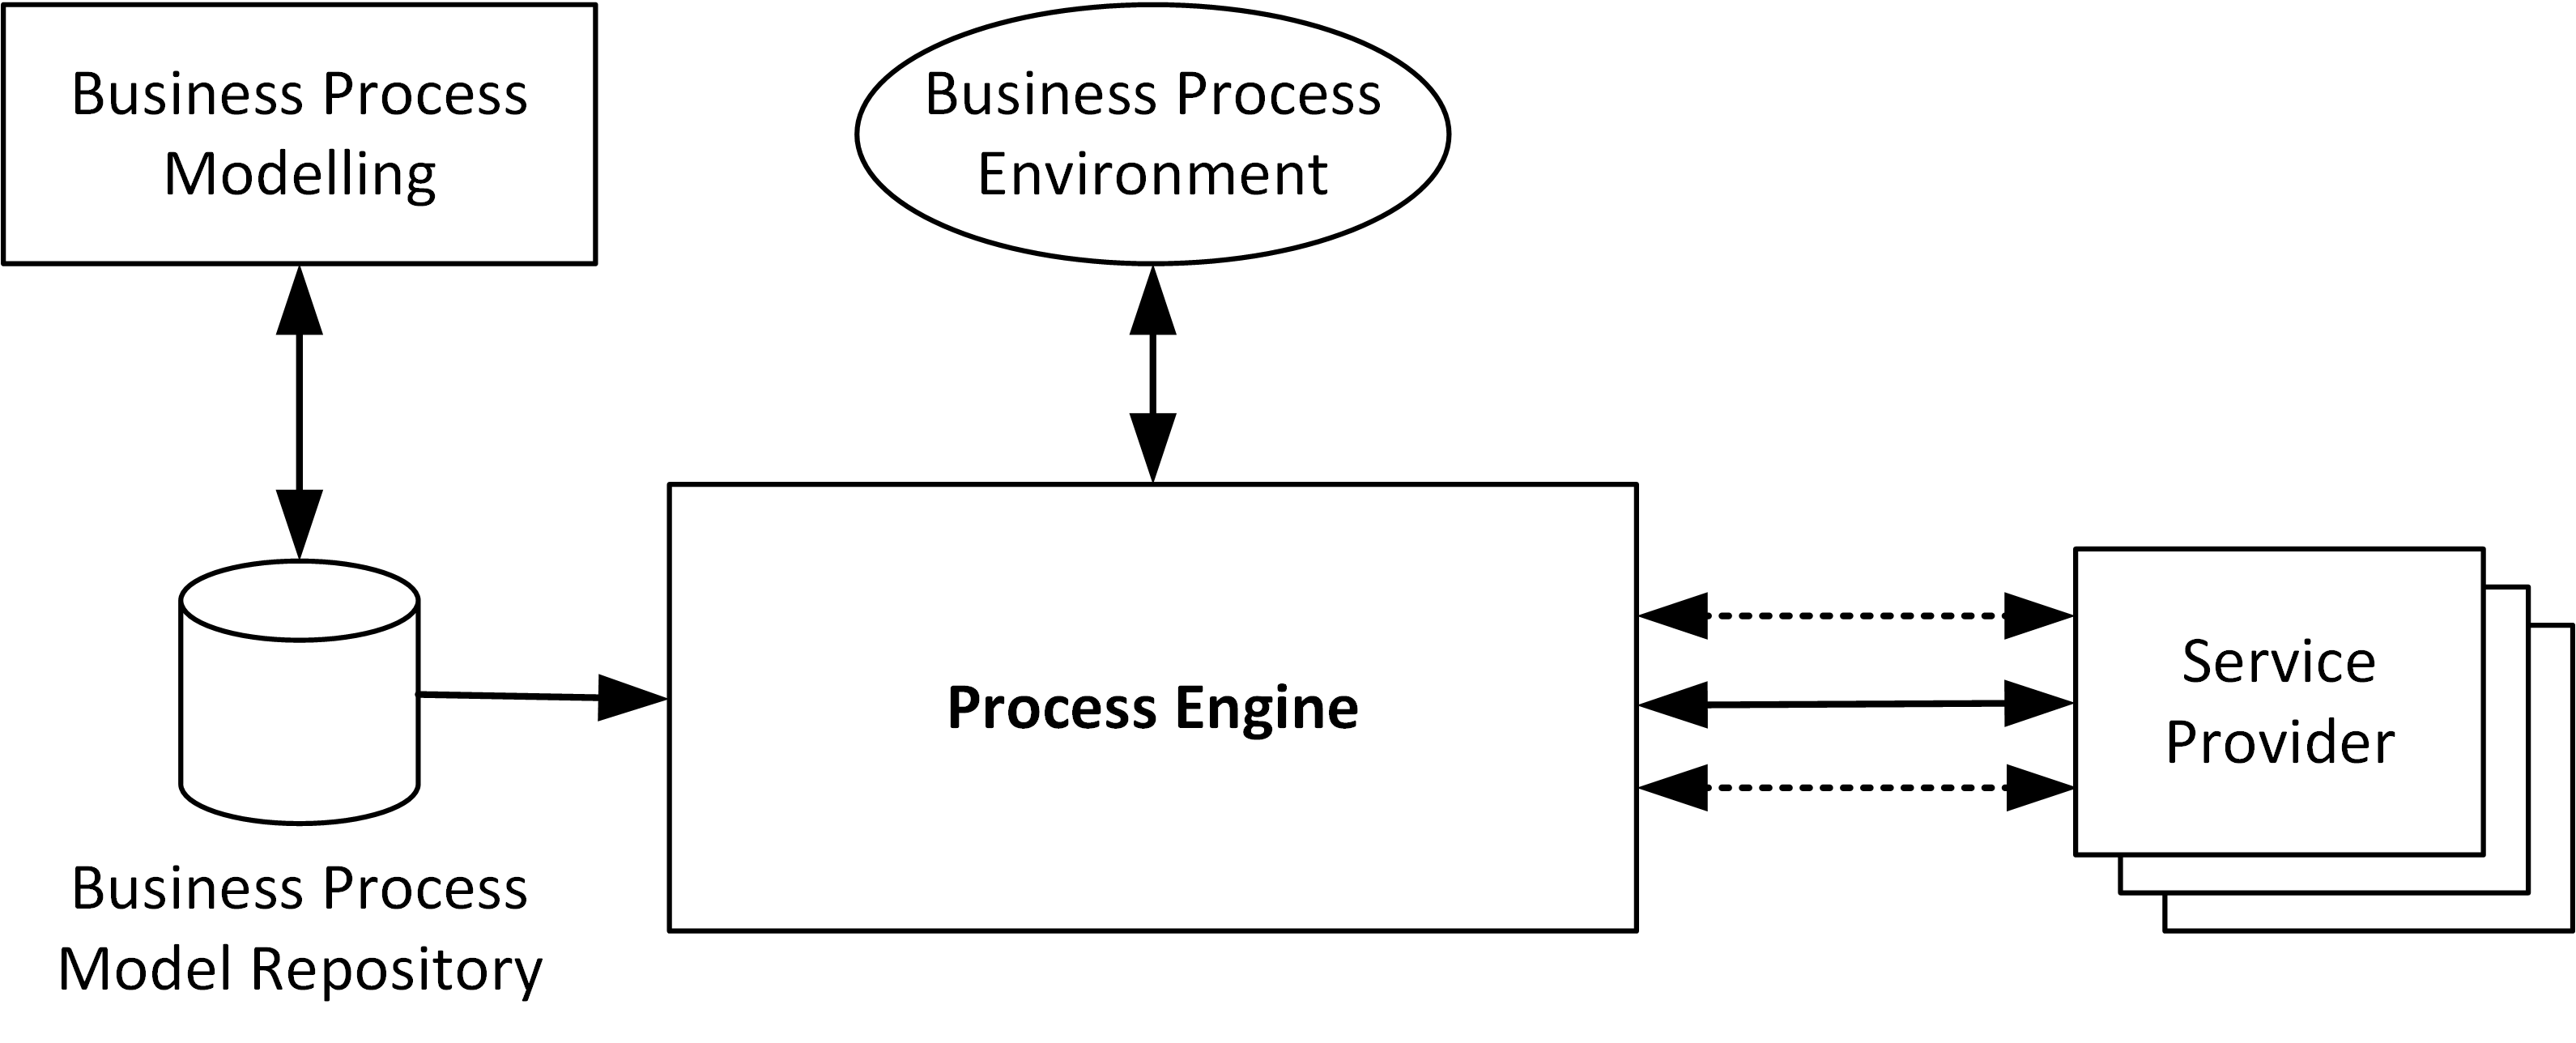
\includegraphics[width=1\linewidth]{chapters/background/bpm-architecture.png}}
	\caption{Business process management systems architecture model (see~\cite{weske:bpm-book},~p.~120)}
	\label{fig:bpm-architecture}
\end{figure}


\paragraph{The Camunda Business Process Engine}\label{ch:bg:camunda}
A large and ever growing number of process engines is available on the market, including solutions from IT giants like SAP, IBM and Oracle.
In this work, \emph{Camunda BPM}~\cite{camunda} has been chosen to illustrate implementations.
As of August 2017, the software product is available in version 7.7.0 and comes in a commercial, regularly updated version and in a free, community-driven solution that is updated with every major release.
Camunda is popular among the research community as the source code is openly available, the product is mature, but actively developed and offers comprehensive support for BPMN 2.0. It is designed to be extensible and easily modifiable to adapt to custom requirements.
\emph{Camunda BPM} comprises a modeling tool, the Camunda process engine core and a number of browser-based user-interfaces to control process enactment and monitor execution state.
\autoref{ch:implementation} will provide further details about the engine architecture and extension mechanisms.


\subsection{Business Process Model and Notation}
Given the general semantics of business processes, a specific modeling notation has to be selected to express an informal process description in a formal, interchangeable way.
Different languages and notations have become available over the years, each serving different specializations.
Kossak~et~al.~\cite{kossak:bpmn2} organize some of the more popular languages as follows: A subset of them are focused on the control flow of business processes, for instance \ac{BPMN}~\cite{bpmnspec}, Yet Another Workflow Language and Petri Nets; some focus on object-orientation, like \ac{UML} activity diagrams and use case diagrams; some are data-flow oriented, e.~g.~the Structured Analysis and Design Technique.
\todo[inline]{references to the other languages}

Among these, the \acs{BPMN} has developed into a widely-adopted industry standard, also becoming ISO-standard in 2013~\cite{iso2013bpmn}.
The standard is developed by the Object Management Group~\cite{omghome} and now available in version 2.0~(January~2011) after being first released in January~2008.
\acs{BPMN} can be understood as an extension to the abstract business process meta model~(\autoref{ch:bg:bpmetamodel}) adding a comprehensive catalog of visual representations and semantic constructs on top of a meta model. Furthermore, one of the most important features of its latest version is the a standardized interchange format provided through an \acs{XML} specification, as \cite{weske:bpm-book} points out.
As emphasized by \citeauthor{Muehlen:2007}~\cite{Muehlen:2007}, the increased expressiveness of modern languages like \acs{BPMN} comes at the cost of an increased complexity. An aspect that, apparently, did not stop it from gaining popularity.

\paragraph{Essential Elements of a BPMN Model}
Following the abstract business process meta model, the core elements in any BPMN model are flow elements~(nodes) and connecting objects~(edges).
Flow elements can be either \textit{Events}, \textit{Activities} or \textit{Gateways}, each of them coming in different versions.
This section will introduce a subset of the elements available through the \acs{BPMN} specification to build the foundation to comprehend the thoughts presented in this work.

\begin{figure}[]
	\myfloatalign
	{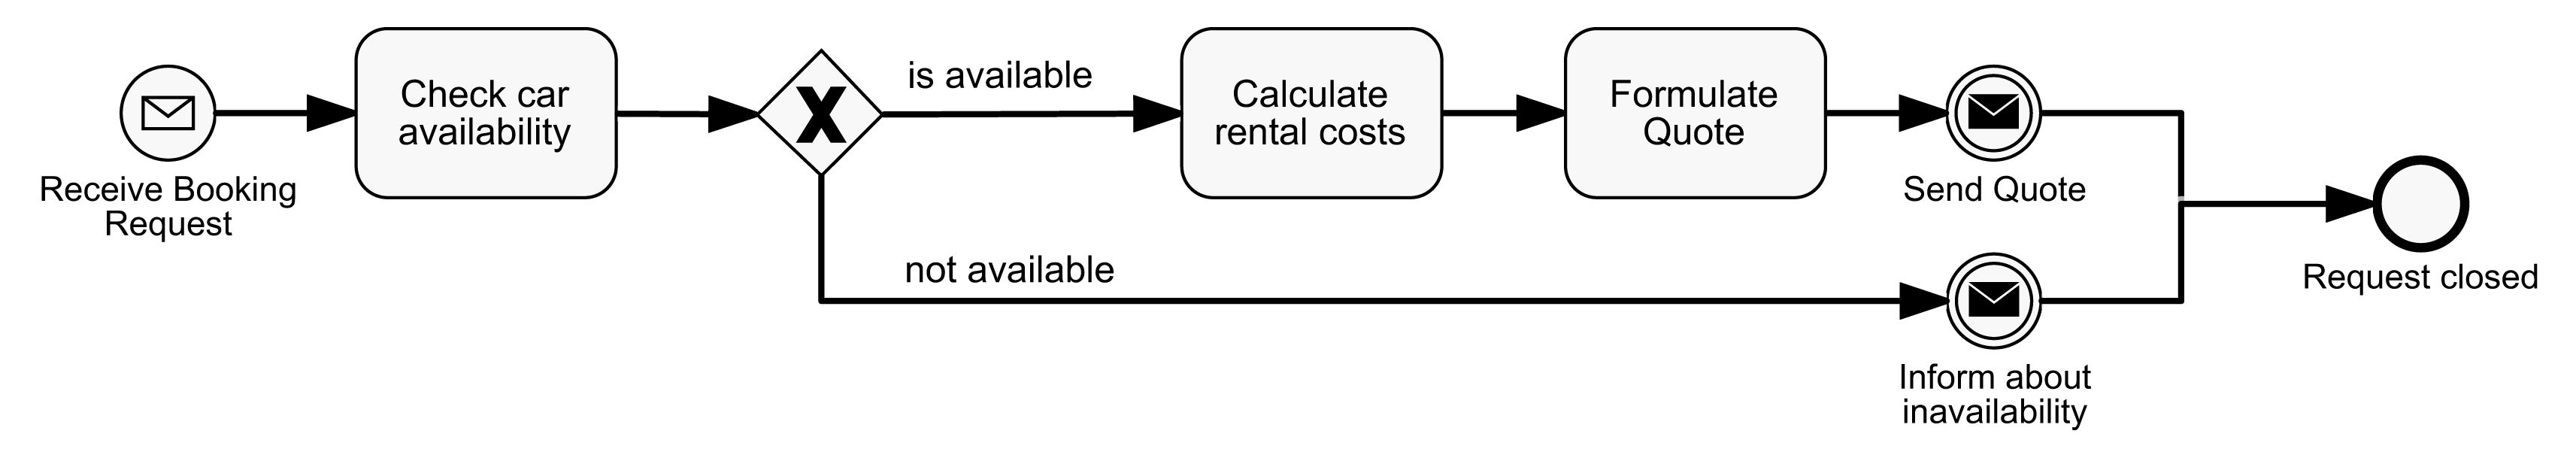
\includegraphics[width=1\linewidth]{chapters/background/intro-rental-car.png}}
	\caption{Simple BPMN model of issuing a quote for car rental}
	\label{fig:simple-bpmn-model}
\end{figure}

\autoref{fig:simple-bpmn-model} shows how a booking request might be handled in a car rental business.
Circular elements represent events, diamond-shaped elements are gateways. Activities are visualized by rectangles with rounded corners.
The given process gets instantiated whenever a booking request request is received from a customer, shown as a Message Start event. 
As a first step, the employee assigned to handle the request must check if the desired car is available. To that follows an exclusive OR-Gateway, distinguishing the further process flow depending on the availability of the car.
If the car is available, the quote must be created in two sequential activities to be then sent out by the \textit{Send Message Event}. If the car is not available, the customer is informed about the closing of his request. 
In either case, the process ends with an \textit{End Event} after the customer was informed about the result of his request.

\todo[inline]{- introduce the other essential elements, types of events}

\paragraph{Process Choreographies}
- talk about how several parties can interact => choreography
- Message
- choreographies

\missingfigure{Sample BPMN choreoraphy model}


\section{Complex Event Processing}
The IT world is facing an exponential increase in the amount of produced data. A significant part of this data are pieces of information about real-life occurrences, such as a current sensor value, an interaction on a website or the location of a vehicle on the road.
We call this kind of strongly time-related information an \textit{Event} and the according computer science field \ac{CEP}~\cite{evtprocessing}.
- events are of a certain type

\todo[inline]{More precisely, Events are defined as follows...}

Four major components take part in an event processing network: (a) An \textit{event producer} provides information to the system, (b) an \textit{event agent} processes the occurring information, so that it can be delivered to the \textit{event consumer}~(c). The components are linked through \textit{event channels}~(d).
Typically, a so-called \textit{\acs{CEP} Engine}~(also: CEP platform) is at the heart of the system, taking the role of an event agent.
Modern CEP platforms are trimmed to maximum efficiency, being able to process hundreds of thousands of events every minute.
Their main purpose is to accept incoming events from event producers, filter and match them according to selection criteria and, finally, derive a new event occurrence to be sent to the registered event consumers.

\paragraph{The publish/subscribe Principle}
In event-based architectures, communication takes place according to the \textit{Publish/Subscribe Principle}.
The concept essentially demands that an event processing middleware publishes events to processes only after they have issued a subscription for these events.
Consequently, there is a strict temporal order between the actions subscribe, consume and un-subscribe. The consumption and un-subscription can only happen after the subscription. Once an un-subscription has been issued, no consumption can follow.~\cite{tanenbaum:2007}

One of the main advantages of this principle is, that the involved parties are \textit{referentially decoupled}. They do not need to explicitly refer to each other, an aspect that is also acknowledged in~\cite{evtprocessing}.
Their decoupled nature facilitates the management and development of event processing networks. Event producers and consumers might change frequently.
Whenever a new event source is available it can be connected to the CEP platform without considering all future consumers. Consumers can subscribe and un-subscribe without influencing the operations on the consumer side.

\missingfigure{pub/sub}

\paragraph{Stream Processing}
To be able to cope with potentially large amounts of data, Complex Event Processing Platforms work on the basis of \textit{stream processing}.
\todo[inline]{'relational' db}
In a traditional database, information is stored for an indefinite amount of time. When a user queries the data store, the system processes the tabular data and calculates the requested result. 
The advantage of this approach is that the user can access historic data at any time, as long as it is not explicitly deleted from the database.
In many occasions, the amount of available data significantly surpasses the storage capacities and that concept can no longer be followed.

Stream processing addresses the mentioned challenge by largely reducing the amount of data that is persisted in the system. Instead, it is the goal to keep only those pieces of information, that are necessary to process a result for currently registered queries.
Incoming data objects, or events in the case of a CEP platform, enter the event stream and are immediately evaluated against all existing query expressions. If the information is not required to process any of the queries, it is deleted instantly.
As a consequence, a certain event can not be part of a query result, if that query has been registered after the occurrence of the event.
In case aggregated information is demanded by the query, the stream processor will internally store aggregated information, but not keep every information that led to the aggregated value.~\cite{streamprocessing} 

\missingfigure{stream processing}

\paragraph{Event Query Languages}
The subscription to an event in a CEP platform is primarily defined by an \textit{Event Query}.
Many modern event query languages are inspired by \acs{SQL}, but cannot be entirely compliant due to the different underlying data processing concept.
When formulating event queries, it is essential to consider the stream processing principle.

For the illustration of the concepts, this thesis relies on the Esper \ac{EPL}~\cite{esperhome}, utilized in Esper event processing engines like the one employed in \autoref{ch:implementation}.

\todo[inline]{a little more on epl, what can it do? windows, joins, filters}

\begin{lstlisting}[language=sql,caption={Sample Query in Esper EPL},label=lst:epl-query-example]
	SELECT time, delay, delayreason
	FROM eurotunnel
	WHERE delay > 30
\end{lstlisting}

\section{Event-driven Business Process Management}
- see opheretzion p.17 and where are we now
- maybe also reference baumgrass paper / GET project | Towards a Methodology for the Engineering
of Event-Driven Process Applications (BG2016)
- + 

- there are 2 use cases for events in bp: 
(1) for process monitoring (=> pe is event producer)
> what's it about
this thesis focusses on (2) as it investigates subscription mechanisms during the execution of a process
%Brandl H.-M. and Guschakowski D. Complex Event Processing in the Context of Business Activity Monitoring

(2) for driving processes (=> pe is event consumer)
%Chandy, K.M. and Schulte, W.R. (2010), Event Processing: Designing IT Systems for Agile Companies, McGraw-Hill, New York, NY
> Event-Driven Process Control (event-driven business process management: where are we now)

- interplay BPT to CEP platforms, a subscription must be issued
- no standard yet available to do subscription in bpmn
- it must be assumed that the subscription is either already active or explicitly modeled in BPMN, e.g. using a service task
- OR given the BPMN spec it is generally assumed that the subscription is executed as soon as en event is enabled
- further analysis of this topic is provided in ...

- Correlating events to process instances

- exercise through one example



